\subsection{Moderne Zahlsysteme}
\subsubsection{Zahlungsabwicklung}

\begin{minipage}{\linewidth}
	\centering
	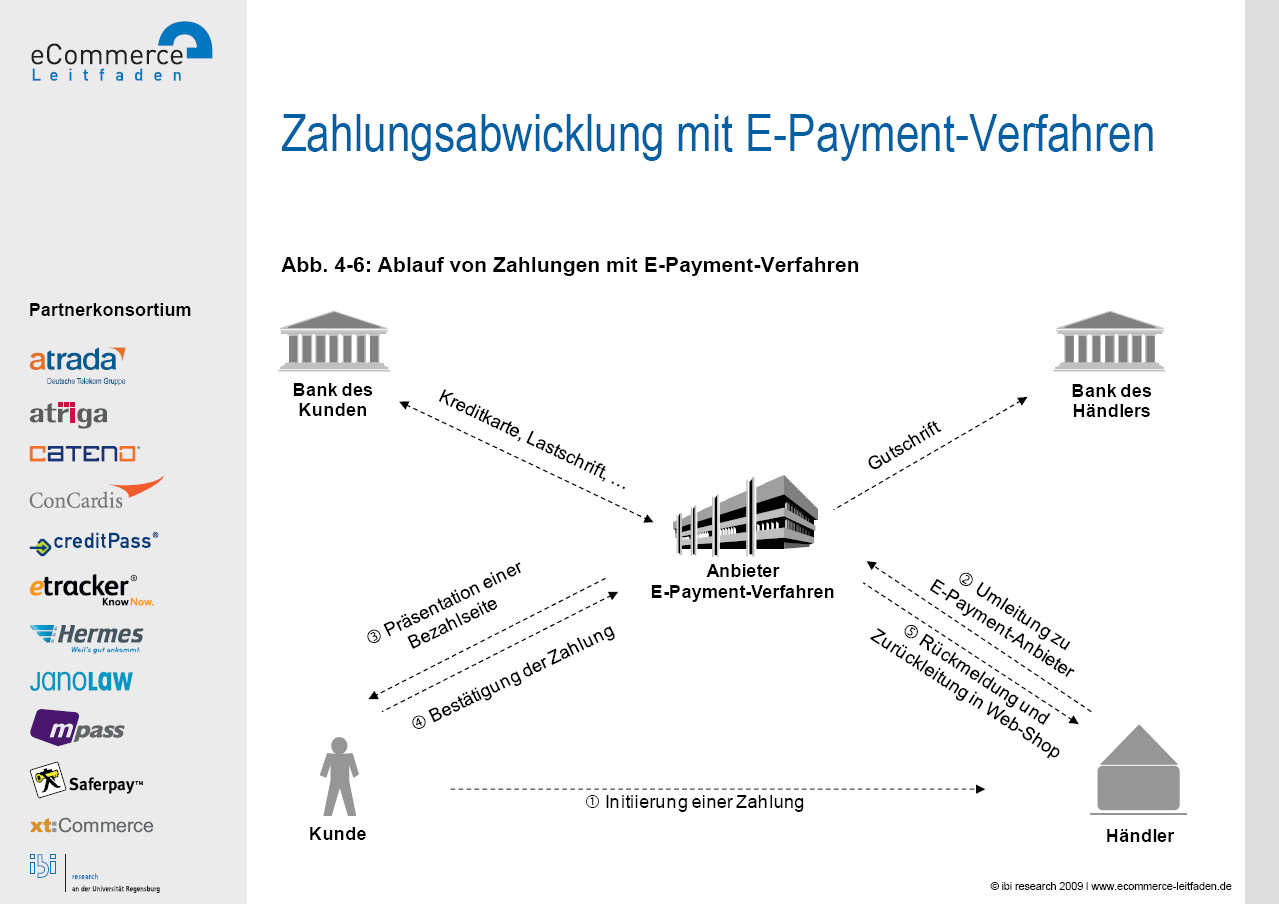
\includegraphics[width=1\linewidth]{images/zahlungsabwicklung}
	\figcaption{Zahlungsabwicklung mit elektronischen Zahlungsverfahren (src: www.ecommerce-leitfaden.de)}
\end{minipage}

Dabei wird die Bezahlung in 5 Schritte unterteilt:

\begin{enumerate}
	\item Zuerst wird die die Zahlung gestartet vom Kunden beim Händler
	\item Der Händler leitet die Anfrage zum E-Payment Anbieter um
	\item der E-Payment Anbieter präsentiert eine von sich bereitgestellte Bezahlseite
	\item Kunde bestätigt die Bezahlung
	\item E-Payment Anbieter gibt Rückmeldung an Händler
\end{enumerate}

Als nächstes werden vom E-Payment Anbieter auf die originären Zahlungsverfahren zurückgegriffen um das Geld vom Kunden anzufragen und anschließlich dem Händler gutzuschreiben. 

\subsubsection{Kategorien}
Es ist grundsätzlich in 4 große Kategorien zu unterscheiden:

\begin{itemize}
	\item E-Mail-basierte Verfahren, wie z. B. PayPal oder Moneybookers, die auf Basis von E-Mail-Adressen und -Kommunikation Zahlungsinformationen austauschen
	\item Karten-basierte Verfahren, wie z. B. die GeldKarte, paysafecard oder MicroMoney, die auf einer Karte des Anbieters des Zahlungsverfahrens basieren
	\item Mobiltelefon-basierte bzw. M-Payment-Verfahren, wie z. B. mpass oder Crandy, die den Besitz einer Mobiltelefonnummer voraussetzen und diese in den Zahlungsablauf einbinden (vgl. das Interview mit Jochen Bornemann, Vodafone, und Michael Kurz, Telefónica O2)
	\item Sonstige Inkasso- und Billing-Verfahren, wie z. B. ClickandBuy, WEB.Cent oder T-Pay, die einzelne Beträge zusammenfassen und dem Händler in einem Betrag auf ein Bankkonto auszahlen
\end{itemize}

Hierbei ist zu beachten, dass jedes Verfahren seine Vor- und Nachteile mit sich bringt und nicht definiert werden kann welches das ''Beste' ist. 

\subsubsection{Anstieg der Popularität}
Daher Online-Shopping immer beliebter wird, werden elektronische Zahlungsmittel auch immer relevanter. In Zukunft werden vor allem traditionelle Banken auch umspringen müssen auf den Trend der Vernetzung.

Zusätzlich zu beachten ist, dadurch das Firmen wie \textbf{PayPal} weit aus mehr Umsätze machen als so manche Banken, müssten diese eigentlich auch staatlich geregelt werden und Fairness für den User gewährleisten. Tatsächlich ist es momentan schon so weit dass staatliche Regelungen bei E-Payment Anbietern durchgezogen werden, aber es sei bekannt dass diese noch stärker angezogen werden.

 
